\begin{frame}{Transactional Datastructures}
\begin{itemize}
    \item<1-> Two transactional datastructures, a Red-Black Tree and a Skiplist have been implemented
    \item<2-> With underlying encounter-order and commit-time transactions taking care of concurrent insertions
    \item<3-> Commit-time transactions cannot successfully be applied to Red-Black Trees, as there are direct dependencies between the transactional writes
    \item<4-> Such restrictions do not exist for Skiplists
    \item<5-> However, the transactional insertion algorithm for both is much simpler than the lock-based or lock-free approaches
\end{itemize}
\end{frame}

\begin{frame}{Red-Black Trees}
\begin{columns}
\column{0.5\textwidth}
\begin{figure}
    \centering
    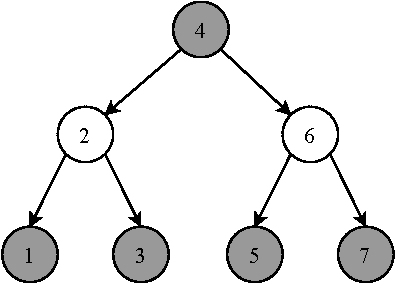
\includegraphics[height=0.5\textheight]{images/rbt.pdf}
\end{figure}

\column{0.5\textwidth}
Properties of Red-Black Trees:
\begin{itemize}
    \item Every node is either red or black
    \item The root and leaf nodes are black
    \item Every red node's children must be black
    \item From each node to its descendant leaves, all paths contain the same number of black nodes
\end{itemize}
\end{columns}
\end{frame}

\begin{frame}{Skiplists}
    

\begin{figure}
    \centering
    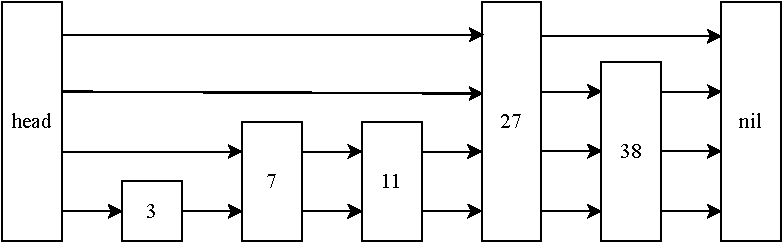
\includegraphics[height=0.35\textheight]{images/skiplist.pdf}
\end{figure}


Properties of Skiplists:
\begin{itemize}
    \item Each node has a certain height $h$ chosen with probability $p$
    \item Nodes are organised into levels of linked lists
    \item Maximum level $L$ is bounded by the number of elements $N$
\end{itemize}

\end{frame}